\documentclass[11pt]{article}

% ------------------------------------------------------------------
% Packages
% ------------------------------------------------------------------
\usepackage[margin=1in]{geometry}
\usepackage{graphicx}       % for \includegraphics
\usepackage{booktabs}       % for professional tables (\toprule, \midrule, \bottomrule)
\usepackage{array}
\usepackage{tabularx}       % tables that stretch to \textwidth
\usepackage{caption}
\usepackage{subcaption}     % side-by-side figures/tables
\usepackage{float}          % [H] placement
\usepackage{siunitx}        % nice number alignment in tables
\usepackage{xcolor}
\usepackage{colortbl}       % row/cell colors
\usepackage{hyperref}
\hypersetup{
    colorlinks=true,
    linkcolor=black,
    urlcolor=blue,
    citecolor=black
}

% A custom row color for alternating rows
\definecolor{lightgray}{gray}{0.93}

% siunitx column type for 4-decimal numbers
\sisetup{round-mode=places, round-precision=4, table-format=1.4}

% ------------------------------------------------------------------
% Title
% ------------------------------------------------------------------
\title{Predicting the Tommy Heinsohn Hustle Award\\
       \large Model Comparison and Results}
\author{Teddy Taussig}
\date{\today}

\begin{document}
\maketitle

% ==================================================================
\section{Overview}
% ==================================================================
This document presents the results of several classification models
trained to predict the recipient of the Tommy Heinsohn Hustle Award on
a per-game basis. We compare regularized logistic regression (ridge,
lasso, elastic net), a decision tree, a random forest, and XGBoost on
the held-out \textbf{2024--25} and \textbf{2025--26} seasons.

% ==================================================================
\section{Model Results}
% ==================================================================
Table~\ref{tab:results} compares every classifier on the held-out
2024--25 and 2025--26 seasons, sorted by Top-1 game accuracy from
highest to lowest.

\begin{table}[H]
    \centering
    \caption{All model results on the 2024--25 and 2025--26 test seasons, ranked by Top-1 game accuracy.}
    \label{tab:results}
    \renewcommand{\arraystretch}{1.25}
    \rowcolors{2}{lightgray}{white}
    \begin{tabular}{l S S S S}
        \toprule
        \textbf{Model} & {\textbf{Top-1 Acc.}} & {\textbf{F1}} & {\textbf{Recall}} & {\textbf{PR-AUC}} \\
        \midrule
        Random forest        & 0.4233 & 0.4233 & 0.4233 & 0.3630 \\
        XGBoost              & 0.3988 & 0.3988 & 0.3988 & 0.3363 \\
        Ridge logistic       & 0.3926 & 0.3926 & 0.3926 & 0.3168 \\
        Elastic-net logistic & 0.3804 & 0.3804 & 0.3804 & 0.3168 \\
        Lasso logistic       & 0.3497 & 0.3497 & 0.3497 & 0.3083 \\
        Decision tree        & 0.3067 & 0.3067 & 0.3067 & 0.2559 \\
        \bottomrule
    \end{tabular}
\end{table}

Table~\ref{tab:results-top1} presents a condensed view with only the
Top-1 game accuracy for each model.

\begin{table}[H]
    \centering
    \caption{Model Top-1 game accuracy on the 2024--25 and 2025--26 test seasons.}
    \label{tab:results-top1}
    \renewcommand{\arraystretch}{1.25}
    \rowcolors{2}{lightgray}{white}
    \begin{tabular}{l S}
        \toprule
        \textbf{Model} & {\textbf{Top-1 Acc.}} \\
        \midrule
        Random forest        & 0.4233 \\
        XGBoost              & 0.3988 \\
        Ridge logistic       & 0.3926 \\
        Elastic-net logistic & 0.3804 \\
        Lasso logistic       & 0.3497 \\
        Decision tree        & 0.3067 \\
        \bottomrule
    \end{tabular}
\end{table}

% ==================================================================
\section{Random Forest Feature Importance}
% ==================================================================
Table~\ref{tab:rf-importance} lists the 15 most important features
from the random-forest classifier (the best-performing model in
Table~\ref{tab:results}).

\begin{table}[H]
    \centering
    \caption{Top 15 feature importances from the random forest classifier.}
    \label{tab:rf-importance}
    \renewcommand{\arraystretch}{1.25}
    \rowcolors{2}{lightgray}{white}
    \begin{tabular}{c l S[table-format=1.6]}
        \toprule
        \textbf{Rank} & \textbf{Feature} & {\textbf{Importance}} \\
        \midrule
        1  & points\_per\_min       & 0.087298 \\
        2  & points                 & 0.075016 \\
        3  & fieldGoalsMade         & 0.069217 \\
        4  & points\_rank           & 0.059923 \\
        5  & usage\_rate            & 0.045435 \\
        6  & fieldGoalsAttempted    & 0.043406 \\
        7  & minutes\_decimal       & 0.039142 \\
        8  & reb\_per\_min          & 0.034920 \\
        9  & threePointersMade      & 0.034456 \\
        10 & impact\_efficiency     & 0.033845 \\
        11 & ast\_per\_min          & 0.032390 \\
        12 & role\_outperformance   & 0.029121 \\
        13 & plusMinusPoints\_rank  & 0.027337 \\
        14 & hustle\_proxy          & 0.027073 \\
        15 & stocks\_per\_min       & 0.026138 \\
        \bottomrule
    \end{tabular}
\end{table}

% ==================================================================
\section{Predicted Tommy Award Picks per Team}
% ==================================================================
Table~\ref{tab:team-picks} lists each opposing team's most-predicted
Tommy Award candidate, with the count of games for which the
random-forest model picked that player as the team's top hustler in
the 2024--25 and 2025--26 seasons.

\begin{table}[H]
    \centering
    \caption{Top predicted hustler per team across the 2024--25 and 2025--26 seasons.}
    \label{tab:team-picks}
    \renewcommand{\arraystretch}{1.2}
    \rowcolors{2}{lightgray}{white}
    \begin{tabular}{l l c c c}
        \toprule
        \textbf{Team} & \textbf{Player} & \textbf{2024--25} & \textbf{2025--26} & \textbf{Total} \\
        \midrule
        Denver Nuggets         & Nikola Jokić            & 50 & 50 & 100 \\
        Milwaukee Bucks        & Giannis Antetokounmpo   & 49 & 29 & 78 \\
        San Antonio Spurs      & Victor Wembanyama       & 29 & 41 & 70 \\
        Oklahoma City Thunder  & Shai Gilgeous-Alexander & 33 & 34 & 67 \\
        Detroit Pistons        & Jalen Duren             & 22 & 38 & 60 \\
        New York Knicks        & Karl-Anthony Towns      & 31 & 26 & 57 \\
        Houston Rockets        & Alperen Sengun          & 31 & 23 & 54 \\
        Phoenix Suns           & Devin Booker            & 29 & 22 & 51 \\
        Los Angeles Clippers   & Ivica Zubac             & 39 & 11 & 50 \\
        Philadelphia 76ers     & Tyrese Maxey            & 22 & 27 & 49 \\
        Los Angeles Lakers     & Luka Dončić             & 10 & 38 & 48 \\
        New Orleans Pelicans   & Zion Williamson         & 18 & 29 & 47 \\
        Golden State Warriors  & Stephen Curry           & 26 & 17 & 43 \\
        Sacramento Kings       & Domantas Sabonis        & 35 &  5 & 40 \\
        Minnesota Timberwolves & Rudy Gobert             & 19 & 21 & 40 \\
        Chicago Bulls          & Nikola Vučević          & 25 & 14 & 39 \\
        Toronto Raptors        & Scottie Barnes          & 14 & 25 & 39 \\
        Cleveland Cavaliers    & Jarrett Allen           & 23 & 15 & 38 \\
        Memphis Grizzlies      & Jaren Jackson Jr.       & 24 & 13 & 37 \\
        Indiana Pacers         & Pascal Siakam           & 17 & 18 & 35 \\
        Portland Trail Blazers & Donovan Clingan         &  9 & 24 & 33 \\
        Miami Heat             & Bam Adebayo             & 16 & 15 & 31 \\
        Orlando Magic          & Paolo Banchero          & 15 & 15 & 30 \\
        Atlanta Hawks          & Trae Young              & 27 &  3 & 30 \\
        Charlotte Hornets      & LaMelo Ball             & 11 & 16 & 27 \\
        Utah Jazz              & Lauri Markkanen         & 11 & 15 & 26 \\
        Washington Wizards     & Alex Sarr               & 10 & 14 & 24 \\
        Dallas Mavericks       & Daniel Gafford          & 15 &  8 & 23 \\
        Brooklyn Nets          & Noah Clowney            &  7 & 10 & 17 \\
        \bottomrule
    \end{tabular}
\end{table}

% ==================================================================
\section{Baseline Figures}
% ==================================================================
Below are the baseline plots exported from the notebooks.

\begin{figure}[H]
    \centering
    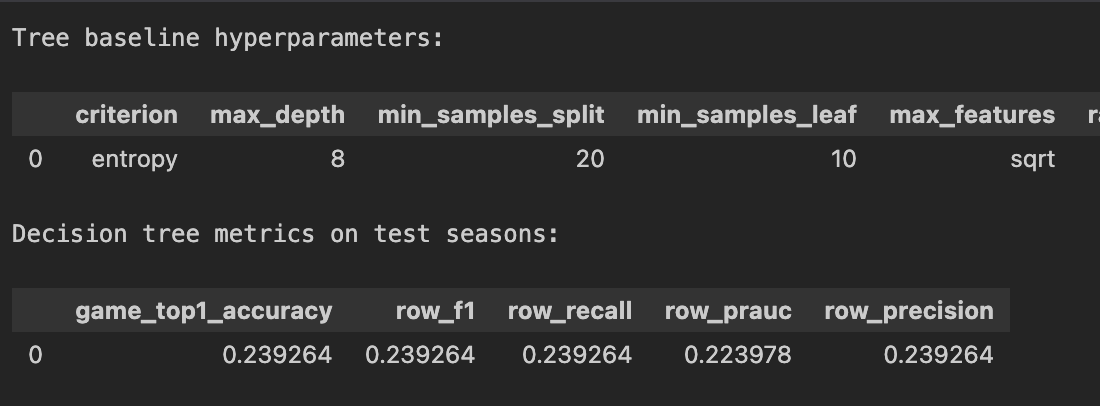
\includegraphics[width=0.8\textwidth]{results_baseline_decision_tree.png}
    \caption{Baseline decision-tree results.}
    \label{fig:dtree-baseline}
\end{figure}

\begin{figure}[H]
    \centering
    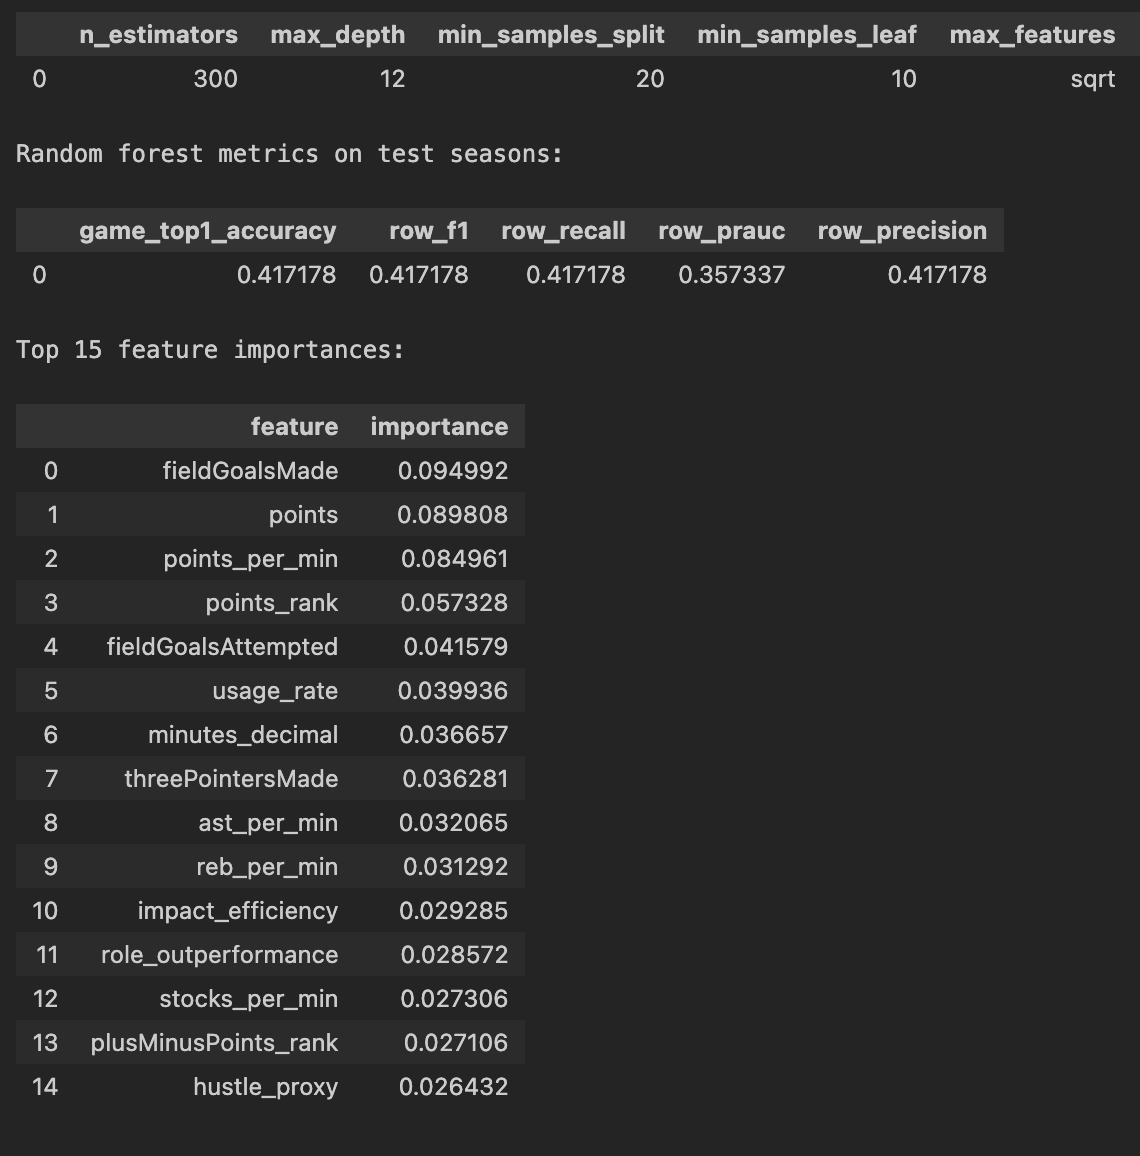
\includegraphics[width=0.8\textwidth]{results_baseline_random_forest.png}
    \caption{Baseline random-forest results.}
    \label{fig:rf-baseline}
\end{figure}

\begin{figure}[H]
    \centering
    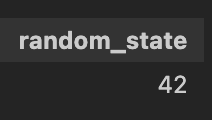
\includegraphics[width=0.6\textwidth]{results_random_state_baseline_decision_tree.png}
    \caption{Decision-tree performance across random states.}
    \label{fig:dtree-random-state}
\end{figure}

% ------------------------------------------------------------------
% Example: two figures side-by-side
% ------------------------------------------------------------------
% \begin{figure}[H]
%     \centering
%     \begin{subfigure}[t]{0.48\textwidth}
%         \centering
%         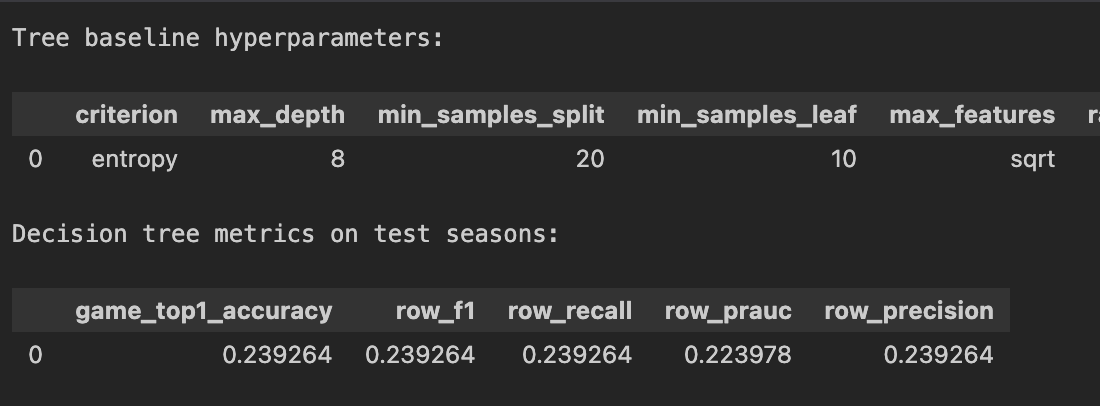
\includegraphics[width=\linewidth]{results_baseline_decision_tree.png}
%         \caption{Decision tree.}
%     \end{subfigure}
%     \hfill
%     \begin{subfigure}[t]{0.48\textwidth}
%         \centering
%         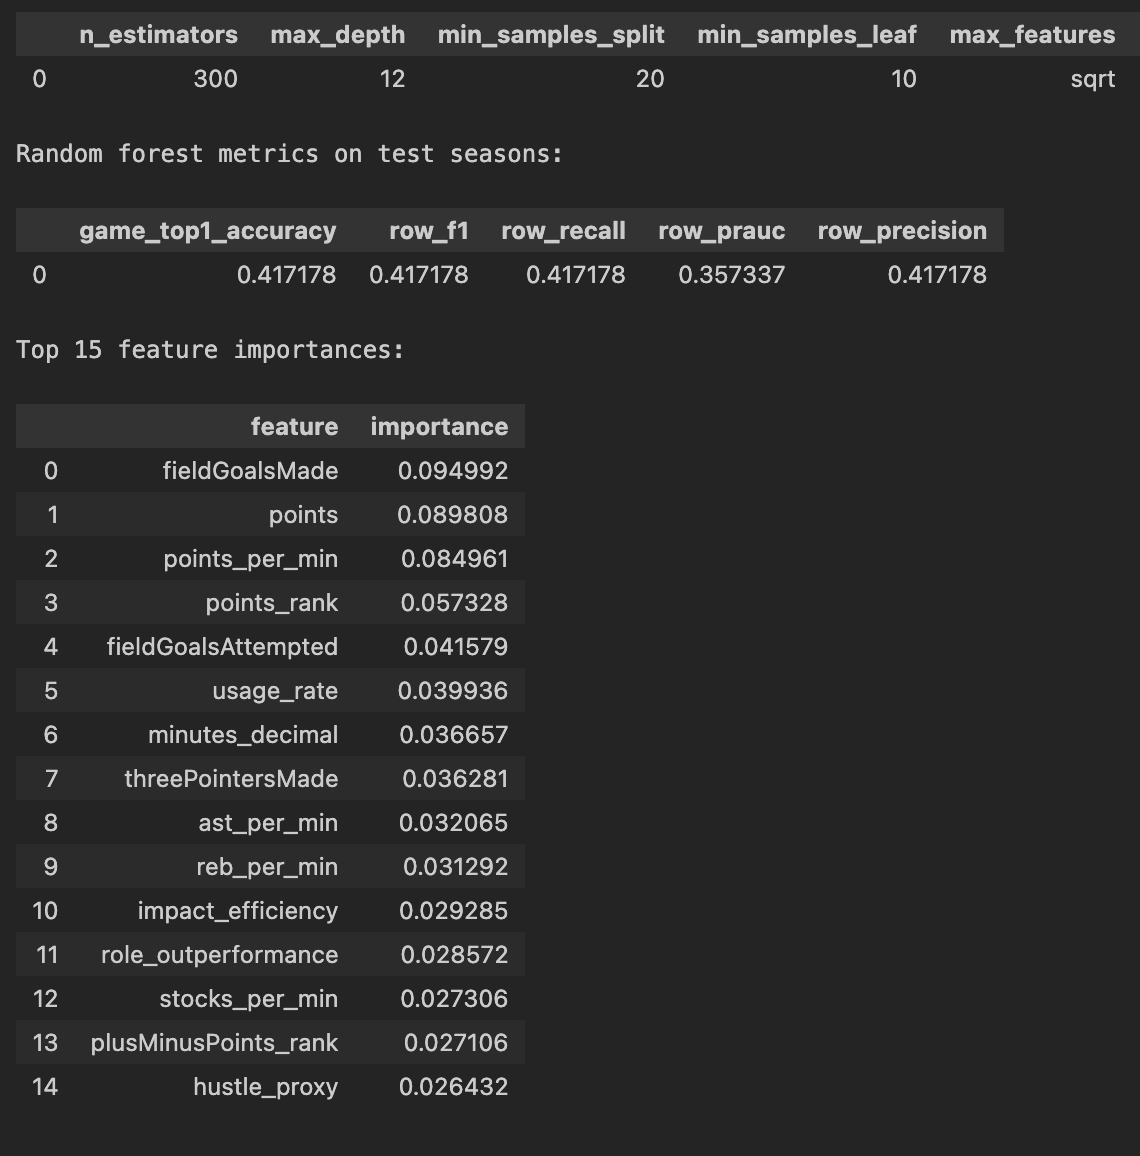
\includegraphics[width=\linewidth]{results_baseline_random_forest.png}
%         \caption{Random forest.}
%     \end{subfigure}
%     \caption{Side-by-side baseline comparisons.}
% \end{figure}

% ==================================================================
\section{Notes}
% ==================================================================
\begin{itemize}
    \item The \texttt{siunitx} package aligns the decimal points so
          numeric columns look clean; adjust \texttt{table-format}
          in the preamble if a column needs more/fewer digits.
    \item To add a new model's row, copy any existing row in
          Table~\ref{tab:results} and replace the numbers.
    \item To add a new figure, drop the image file into the same
          folder as this \texttt{.tex} file and copy a
          \verb|\begin{figure}...\end{figure}| block.
\end{itemize}

\end{document}
